\documentclass[usenames,dvipsnames,tikz]{standalone}
\usetikzlibrary{shapes.geometric}
\usepackage{xcolor}
\colorlet{tBlue}{RoyalBlue!35!Cerulean}
\colorlet{tRed}{Red}
\begin{document}
	
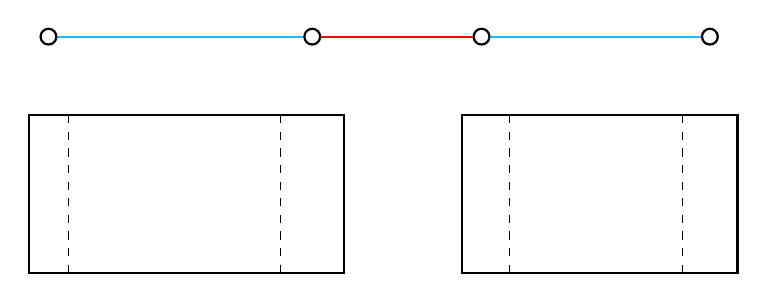
\begin{tikzpicture}
%\draw [help lines] (-1,-2) grid (11,5);

\draw [tBlue, thick] (0.25,3) -- (3.75,3);
\draw [tBlue, thick] (5.75,3) -- (8.65,3);
\draw [tRed, thick] (3.6,3) -- (5.75,3);

\draw [fill=white, thick] (0.25,3) circle [radius = 0.1];
\draw [fill=white, thick] (3.6,3) circle [radius = 0.1];
\draw [fill=white, thick] (5.75,3) circle [radius = 0.1];
\draw [fill=white, thick] (8.65,3) circle [radius = 0.1];


\draw [thick] (0,0) rectangle (4,2);
\draw [thick] (5.5,0) rectangle (9,2);

\draw [dashed] (0.5,0) -- (0.5,2);
\draw [dashed] (3.2,0) -- (3.2,2);

\draw [dashed] (6.1,0) -- (6.1,2);
\draw [dashed] (8.3,0) -- (8.3,2);



\end{tikzpicture}
	
\end{document}